% This template was initially provided by Dulip Withanage.
% Modifications for the database systems research group
% were made by Conny Junghans, Jannik Stroetgen and Michael Gertz

\documentclass[
     12pt,         % font size
     a4paper,      % paper format
     BCOR10mm,     % binding correction
     DIV14,        % stripe size for margin calculation
     ]{article}

%%%%%%%%%%%%%%%%%%%%%%%%%%%%%%%%%%%%%%%%%%%%%%%%%%%%%%%%%%%%

% PACKAGES:

% Use English :
\usepackage[english]{babel}
% Input and font encoding
\usepackage[latin1]{inputenc}
\usepackage[T1]{fontenc}
\usepackage{lmodern}
% Index-generation
\usepackage{makeidx}
% Einbinden von URLs:
\usepackage{url}
% Special \LaTex symbols (e.g. \BibTeX):
%\usepackage{doc}
% Include Graphic-files:
\usepackage{graphicx}
% Include doc++ generated tex-files:
%\usepackage{docxx}
\usepackage[english]{babel}
\usepackage[
backend=biber
,style=ieee
,backref
,defernumbers=true
]{biblatex}

\addbibresource[datatype=bibtex]{references.bib}

% Fuer anderthalbzeiligen Textsatz
\usepackage{setspace}

% hyperrefs in the documents
\PassOptionsToPackage{hyphens}{url}\usepackage[bookmarks=true,colorlinks,pdfpagelabels,pdfstartview = FitH,bookmarksopen = true,bookmarksnumbered = true,linkcolor = black,plainpages = false,hypertexnames = false,citecolor = black,urlcolor=black]{hyperref}
%\usepackage{hyperref}

% Choose language
\newcommand{\setlang}[1]{\selectlanguage{#1}\nonfrenchspacing}

%%%%%%%%%%%%%%%%%%%%%%%%%%%%%%%%%%%%%%%%%%%%%%%%%%%%%%%%%%%%

% OTHER SETTINGS:

\usepackage{csquotes}
\usepackage{float}
\usepackage{longtable}
\usepackage{listings}
\usepackage{color}

\definecolor{dkgreen}{rgb}{0,0.6,0}
\definecolor{gray}{rgb}{0.5,0.5,0.5}
\definecolor{mauve}{rgb}{0.58,0,0.82}

\lstset{
	frame=tb,
	language=Java,
	aboveskip=3mm,
	belowskip=3mm,
	showstringspaces=false,
	columns=flexible,
	basicstyle={\small\ttfamily},
	morekeywords={UC, context, pre, @pre, post, and, or, not, implies, forall, exists},
	numbers=none,
	numberstyle=\tiny\color{gray},
	keywordstyle=\color{blue},
	commentstyle=\color{dkgreen},
	stringstyle=\color{mauve},
	breaklines=true,
	breakatwhitespace=true,
	tabsize=3
}

%%%%%%%%%%%%%%%%%%%%%%%%%%%%%%%%%%%%%%%%%%%%%%%%%%%%%%%%%%%%

% DOCUMENT HEADER:

\begin{document}

\pagenumbering{roman} 
\begin{titlepage}

\vspace*{1cm}
\begin{center}
\textbf{ 
\Large Heidelberg University\\
\smallskip
\Large Institute of Computer Science\\
\smallskip
\Large Software Engineering Group\\
\smallskip
}

\vspace{3cm}

\textbf{\large Better Software Through Systematic Testing}

\vspace{0.5\baselineskip}
{\huge
\textbf{Literature Synthesis}
}
\vspace{0.5cm}

\url{https://github.com/fidsusj/SWE-Seminar}

\vspace{0.5cm}

{\small
	\begin{tabular}[l]{ll}
		Felix Hausberger, 3661293,\\
		Applied Computer Science\\
		eb260@stud.uni-heidelberg.de\\
	\end{tabular}
}
\end{center}



\end{titlepage}

%%%%%%%%%%%%%%%%%%%%%%%%%%%%%%%%%%%%%%%%%%%%%%%%%%%%%%%%%%%%

% DOCUMENT CONTENT:

\pagenumbering{arabic} 

% This template was initially provided by Dulip Withanage.
% Modifications for the database systems research group
% were made by Conny Junghans, Jannik Stroetgen and Michael Gertz

\documentclass[
     12pt,         % font size
     a4paper,      % paper format
     BCOR10mm,     % binding correction
     DIV14,        % stripe size for margin calculation
     ]{article}

%%%%%%%%%%%%%%%%%%%%%%%%%%%%%%%%%%%%%%%%%%%%%%%%%%%%%%%%%%%%

% PACKAGES:

% Use English :
\usepackage[english]{babel}
% Input and font encoding
\usepackage[latin1]{inputenc}
\usepackage[T1]{fontenc}
\usepackage{lmodern}
% Index-generation
\usepackage{makeidx}
% Einbinden von URLs:
\usepackage{url}
% Special \LaTex symbols (e.g. \BibTeX):
%\usepackage{doc}
% Include Graphic-files:
\usepackage{graphicx}
% Include doc++ generated tex-files:
%\usepackage{docxx}
\usepackage[english]{babel}
\usepackage[
backend=biber
,style=ieee
,backref
,defernumbers=true
]{biblatex}

\addbibresource[datatype=bibtex]{references.bib}

% Fuer anderthalbzeiligen Textsatz
\usepackage{setspace}

% hyperrefs in the documents
\PassOptionsToPackage{hyphens}{url}\usepackage[bookmarks=true,colorlinks,pdfpagelabels,pdfstartview = FitH,bookmarksopen = true,bookmarksnumbered = true,linkcolor = black,plainpages = false,hypertexnames = false,citecolor = black,urlcolor=black]{hyperref}
%\usepackage{hyperref}

% Choose language
\newcommand{\setlang}[1]{\selectlanguage{#1}\nonfrenchspacing}

%%%%%%%%%%%%%%%%%%%%%%%%%%%%%%%%%%%%%%%%%%%%%%%%%%%%%%%%%%%%

% OTHER SETTINGS:

\usepackage{csquotes}
\usepackage{float}
\usepackage{longtable}
\usepackage{listings}
\usepackage{color}

\definecolor{dkgreen}{rgb}{0,0.6,0}
\definecolor{gray}{rgb}{0.5,0.5,0.5}
\definecolor{mauve}{rgb}{0.58,0,0.82}

\lstset{
	frame=tb,
	language=Java,
	aboveskip=3mm,
	belowskip=3mm,
	showstringspaces=false,
	columns=flexible,
	basicstyle={\small\ttfamily},
	morekeywords={UC, context, pre, @pre, post, and, or, not, implies, forall, exists},
	numbers=none,
	numberstyle=\tiny\color{gray},
	keywordstyle=\color{blue},
	commentstyle=\color{dkgreen},
	stringstyle=\color{mauve},
	breaklines=true,
	breakatwhitespace=true,
	tabsize=3
}

%%%%%%%%%%%%%%%%%%%%%%%%%%%%%%%%%%%%%%%%%%%%%%%%%%%%%%%%%%%%

% DOCUMENT HEADER:

\begin{document}

\pagenumbering{roman} 
\begin{titlepage}

\vspace*{1cm}
\begin{center}
\textbf{ 
\Large Heidelberg University\\
\smallskip
\Large Institute of Computer Science\\
\smallskip
\Large Software Engineering Group\\
\smallskip
}

\vspace{3cm}

\textbf{\large Better Software Through Systematic Testing}

\vspace{0.5\baselineskip}
{\huge
\textbf{Literature Synthesis}
}
\vspace{0.5cm}

\url{https://github.com/fidsusj/SWE-Seminar}

\vspace{0.5cm}

{\small
	\begin{tabular}[l]{ll}
		Felix Hausberger, 3661293,\\
		Applied Computer Science\\
		eb260@stud.uni-heidelberg.de\\
	\end{tabular}
}
\end{center}



\end{titlepage}

%%%%%%%%%%%%%%%%%%%%%%%%%%%%%%%%%%%%%%%%%%%%%%%%%%%%%%%%%%%%

% DOCUMENT CONTENT:

\pagenumbering{arabic} 

% This template was initially provided by Dulip Withanage.
% Modifications for the database systems research group
% were made by Conny Junghans, Jannik Stroetgen and Michael Gertz

\documentclass[
     12pt,         % font size
     a4paper,      % paper format
     BCOR10mm,     % binding correction
     DIV14,        % stripe size for margin calculation
     ]{article}

%%%%%%%%%%%%%%%%%%%%%%%%%%%%%%%%%%%%%%%%%%%%%%%%%%%%%%%%%%%%

% PACKAGES:

% Use English :
\usepackage[english]{babel}
% Input and font encoding
\usepackage[latin1]{inputenc}
\usepackage[T1]{fontenc}
\usepackage{lmodern}
% Index-generation
\usepackage{makeidx}
% Einbinden von URLs:
\usepackage{url}
% Special \LaTex symbols (e.g. \BibTeX):
%\usepackage{doc}
% Include Graphic-files:
\usepackage{graphicx}
% Include doc++ generated tex-files:
%\usepackage{docxx}
\usepackage[english]{babel}
\usepackage[
backend=biber
,style=ieee
,backref
,defernumbers=true
]{biblatex}

\addbibresource[datatype=bibtex]{references.bib}

% Fuer anderthalbzeiligen Textsatz
\usepackage{setspace}

% hyperrefs in the documents
\PassOptionsToPackage{hyphens}{url}\usepackage[bookmarks=true,colorlinks,pdfpagelabels,pdfstartview = FitH,bookmarksopen = true,bookmarksnumbered = true,linkcolor = black,plainpages = false,hypertexnames = false,citecolor = black,urlcolor=black]{hyperref}
%\usepackage{hyperref}

% Choose language
\newcommand{\setlang}[1]{\selectlanguage{#1}\nonfrenchspacing}

%%%%%%%%%%%%%%%%%%%%%%%%%%%%%%%%%%%%%%%%%%%%%%%%%%%%%%%%%%%%

% OTHER SETTINGS:

\usepackage{csquotes}
\usepackage{float}
\usepackage{longtable}
\usepackage{listings}
\usepackage{color}

\definecolor{dkgreen}{rgb}{0,0.6,0}
\definecolor{gray}{rgb}{0.5,0.5,0.5}
\definecolor{mauve}{rgb}{0.58,0,0.82}

\lstset{
	frame=tb,
	language=Java,
	aboveskip=3mm,
	belowskip=3mm,
	showstringspaces=false,
	columns=flexible,
	basicstyle={\small\ttfamily},
	morekeywords={UC, context, pre, @pre, post, and, or, not, implies, forall, exists},
	numbers=none,
	numberstyle=\tiny\color{gray},
	keywordstyle=\color{blue},
	commentstyle=\color{dkgreen},
	stringstyle=\color{mauve},
	breaklines=true,
	breakatwhitespace=true,
	tabsize=3
}

%%%%%%%%%%%%%%%%%%%%%%%%%%%%%%%%%%%%%%%%%%%%%%%%%%%%%%%%%%%%

% DOCUMENT HEADER:

\begin{document}

\pagenumbering{roman} 
\begin{titlepage}

\vspace*{1cm}
\begin{center}
\textbf{ 
\Large Heidelberg University\\
\smallskip
\Large Institute of Computer Science\\
\smallskip
\Large Software Engineering Group\\
\smallskip
}

\vspace{3cm}

\textbf{\large Better Software Through Systematic Testing}

\vspace{0.5\baselineskip}
{\huge
\textbf{Literature Synthesis}
}
\vspace{0.5cm}

\url{https://github.com/fidsusj/SWE-Seminar}

\vspace{0.5cm}

{\small
	\begin{tabular}[l]{ll}
		Felix Hausberger, 3661293,\\
		Applied Computer Science\\
		eb260@stud.uni-heidelberg.de\\
	\end{tabular}
}
\end{center}



\end{titlepage}

%%%%%%%%%%%%%%%%%%%%%%%%%%%%%%%%%%%%%%%%%%%%%%%%%%%%%%%%%%%%

% DOCUMENT CONTENT:

\pagenumbering{arabic} 

% This template was initially provided by Dulip Withanage.
% Modifications for the database systems research group
% were made by Conny Junghans, Jannik Stroetgen and Michael Gertz

\documentclass[
     12pt,         % font size
     a4paper,      % paper format
     BCOR10mm,     % binding correction
     DIV14,        % stripe size for margin calculation
     ]{article}

%%%%%%%%%%%%%%%%%%%%%%%%%%%%%%%%%%%%%%%%%%%%%%%%%%%%%%%%%%%%

% PACKAGES:

% Use English :
\usepackage[english]{babel}
% Input and font encoding
\usepackage[latin1]{inputenc}
\usepackage[T1]{fontenc}
\usepackage{lmodern}
% Index-generation
\usepackage{makeidx}
% Einbinden von URLs:
\usepackage{url}
% Special \LaTex symbols (e.g. \BibTeX):
%\usepackage{doc}
% Include Graphic-files:
\usepackage{graphicx}
% Include doc++ generated tex-files:
%\usepackage{docxx}
\usepackage[english]{babel}
\usepackage[
backend=biber
,style=ieee
,backref
,defernumbers=true
]{biblatex}

\addbibresource[datatype=bibtex]{references.bib}

% Fuer anderthalbzeiligen Textsatz
\usepackage{setspace}

% hyperrefs in the documents
\PassOptionsToPackage{hyphens}{url}\usepackage[bookmarks=true,colorlinks,pdfpagelabels,pdfstartview = FitH,bookmarksopen = true,bookmarksnumbered = true,linkcolor = black,plainpages = false,hypertexnames = false,citecolor = black,urlcolor=black]{hyperref}
%\usepackage{hyperref}

% Choose language
\newcommand{\setlang}[1]{\selectlanguage{#1}\nonfrenchspacing}

%%%%%%%%%%%%%%%%%%%%%%%%%%%%%%%%%%%%%%%%%%%%%%%%%%%%%%%%%%%%

% OTHER SETTINGS:

\usepackage{csquotes}
\usepackage{float}
\usepackage{longtable}
\usepackage{listings}
\usepackage{color}

\definecolor{dkgreen}{rgb}{0,0.6,0}
\definecolor{gray}{rgb}{0.5,0.5,0.5}
\definecolor{mauve}{rgb}{0.58,0,0.82}

\lstset{
	frame=tb,
	language=Java,
	aboveskip=3mm,
	belowskip=3mm,
	showstringspaces=false,
	columns=flexible,
	basicstyle={\small\ttfamily},
	morekeywords={UC, context, pre, @pre, post, and, or, not, implies, forall, exists},
	numbers=none,
	numberstyle=\tiny\color{gray},
	keywordstyle=\color{blue},
	commentstyle=\color{dkgreen},
	stringstyle=\color{mauve},
	breaklines=true,
	breakatwhitespace=true,
	tabsize=3
}

%%%%%%%%%%%%%%%%%%%%%%%%%%%%%%%%%%%%%%%%%%%%%%%%%%%%%%%%%%%%

% DOCUMENT HEADER:

\begin{document}

\pagenumbering{roman} 
\begin{titlepage}

\vspace*{1cm}
\begin{center}
\textbf{ 
\Large Heidelberg University\\
\smallskip
\Large Institute of Computer Science\\
\smallskip
\Large Software Engineering Group\\
\smallskip
}

\vspace{3cm}

\textbf{\large Better Software Through Systematic Testing}

\vspace{0.5\baselineskip}
{\huge
\textbf{Literature Synthesis}
}
\vspace{0.5cm}

\url{https://github.com/fidsusj/SWE-Seminar}

\vspace{0.5cm}

{\small
	\begin{tabular}[l]{ll}
		Felix Hausberger, 3661293,\\
		Applied Computer Science\\
		eb260@stud.uni-heidelberg.de\\
	\end{tabular}
}
\end{center}



\end{titlepage}

%%%%%%%%%%%%%%%%%%%%%%%%%%%%%%%%%%%%%%%%%%%%%%%%%%%%%%%%%%%%

% DOCUMENT CONTENT:

\pagenumbering{arabic} 

\input{content/synthesis}
\input{content/example}


%%%%%%%%%%%%%%%%%%%%%%%%%%%%%%%%%%%%%%%%%%%%%%%%%%%%%%%%%%%%

% REFERENCES:
\newpage
\printbibliography

\end{document}

\section{Example}

In this chapter both approaches should be demonstrated within the example of a movie management software.  

\subsection{Automatic Test Generation: A Use Case Driven Approach}

In the first step the test objectives have to be derived. Therefore we define the use cases and their contracts as requirement-level logical expressions. Only the use cases that really impact the state of the transition system were specified for this example. The notation used is equal to the one proposed in the paper. 

\begin{lstlisting}
UC createMovie(m: movie)
post createdMovie(m)

UC createLinkedPerformer(p: performer, m: movie)
pre createdMovie(m)
post createdPerformer(p) and createdLink(p,m)

UC rateMovie(m: movie)
pre createdMovie(m)
post calculatedOverallRating(m)

UC ratePerformer(p: performer)
pre createdPerformer(p)
post forall(m: movie){ createdLink(p,m)@pre implies calculatedOverallRating(m) }

UC linkExistingMovie(m: movie, p: performer)
pre createdMovie(m) and createdPerformer(p)
post not createdLink(p,m)@pre implies (createdLink(p,m) and calculatedOverallRating(m))

UC linkExistingPerformer(m: movie, p: performer)
pre createdMovie(m) and createdPerformer(p)
post not createdLink(p,m)@pre implies (createdLink(p,m) and calculatedOverallRating(m))

UC unlinkMovie(m: movie, p: performer)
pre createdMovie(m) and createdPerformer(p) and createdLink(p,m)
post calculatedOverallRating(m) and not createdLink(p,m) and not exists(m2: movie){ createdLink(p,m2) }@pre implies not createdPerformer(p)

UC unlinkPerformer(m: movie, p: performer)
pre createdMovie(m) and createdPerformer(p) and createdLink(p,m)
post calculatedOverallRating(m) and not createdLink(p,m) and not exists(m2: movie){ createdLink(p,m2) }@pre implies not createdPerformer(p)

UC removeMovie(m: movie)
pre createdMovie(m)
post not createdMovie(m) and forall(p: performer){ not createdLink(p,m) } and not exist(m2: movie){ createdLink(p,m2) }@pre implies not createdPerformer(p)

UC removePerformer(p: performer)
pre createdPerformer(p)
post not createdPerformer(p) and forall(m: movie){ not createdLink(p,m) }

\end{lstlisting}

After that the UCSystem tool should build the UCTS (\autoref{ucts}) through exhaustive simulation. The pool of parameters was restricted to one movie and performer to avoid a combinatorical explosion for this example. Furthermore the predicate calculatedOverallRating is no longer considered. Note that only predicates that evaluate to true are listed in the states as in the original paper. 

\begin{figure}[h]
	\centering
	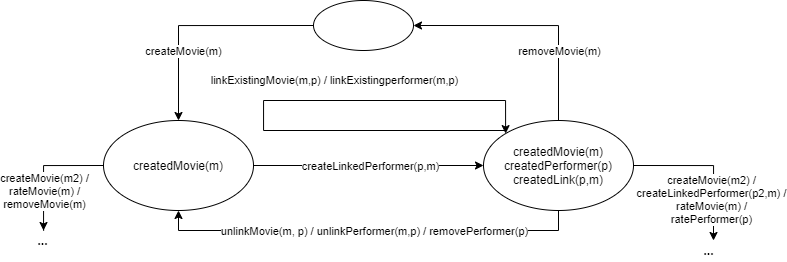
\includegraphics[width=1.0\textwidth]{img/ucts.png}
	\label{ucts}
\end{figure}

Depending on the selected coverage criterion, we receive different test objectives. How many test objectives are derived depends on the internal implementation of UCSystem and cannot be predicted for this example. Let's assume that one test objective is the test path createMovie(m) -> createLinkedPerformer(p,m) -> unlinkMovie(m). 




\subsection{An Automated Approach to System Testing based on Scenarios and Operations Contracts}


%%%%%%%%%%%%%%%%%%%%%%%%%%%%%%%%%%%%%%%%%%%%%%%%%%%%%%%%%%%%

% REFERENCES:
\newpage
\printbibliography

\end{document}

\section{Example}

In this chapter both approaches should be demonstrated within the example of a movie management software.  

\subsection{Automatic Test Generation: A Use Case Driven Approach}

In the first step the test objectives have to be derived. Therefore we define the use cases and their contracts as requirement-level logical expressions. Only the use cases that really impact the state of the transition system were specified for this example. The notation used is equal to the one proposed in the paper. 

\begin{lstlisting}
UC createMovie(m: movie)
post createdMovie(m)

UC createLinkedPerformer(p: performer, m: movie)
pre createdMovie(m)
post createdPerformer(p) and createdLink(p,m)

UC rateMovie(m: movie)
pre createdMovie(m)
post calculatedOverallRating(m)

UC ratePerformer(p: performer)
pre createdPerformer(p)
post forall(m: movie){ createdLink(p,m)@pre implies calculatedOverallRating(m) }

UC linkExistingMovie(m: movie, p: performer)
pre createdMovie(m) and createdPerformer(p)
post not createdLink(p,m)@pre implies (createdLink(p,m) and calculatedOverallRating(m))

UC linkExistingPerformer(m: movie, p: performer)
pre createdMovie(m) and createdPerformer(p)
post not createdLink(p,m)@pre implies (createdLink(p,m) and calculatedOverallRating(m))

UC unlinkMovie(m: movie, p: performer)
pre createdMovie(m) and createdPerformer(p) and createdLink(p,m)
post calculatedOverallRating(m) and not createdLink(p,m) and not exists(m2: movie){ createdLink(p,m2) }@pre implies not createdPerformer(p)

UC unlinkPerformer(m: movie, p: performer)
pre createdMovie(m) and createdPerformer(p) and createdLink(p,m)
post calculatedOverallRating(m) and not createdLink(p,m) and not exists(m2: movie){ createdLink(p,m2) }@pre implies not createdPerformer(p)

UC removeMovie(m: movie)
pre createdMovie(m)
post not createdMovie(m) and forall(p: performer){ not createdLink(p,m) } and not exist(m2: movie){ createdLink(p,m2) }@pre implies not createdPerformer(p)

UC removePerformer(p: performer)
pre createdPerformer(p)
post not createdPerformer(p) and forall(m: movie){ not createdLink(p,m) }

\end{lstlisting}

After that the UCSystem tool should build the UCTS (\autoref{ucts}) through exhaustive simulation. The pool of parameters was restricted to one movie and performer to avoid a combinatorical explosion for this example. Furthermore the predicate calculatedOverallRating is no longer considered. Note that only predicates that evaluate to true are listed in the states as in the original paper. 

\begin{figure}[h]
	\centering
	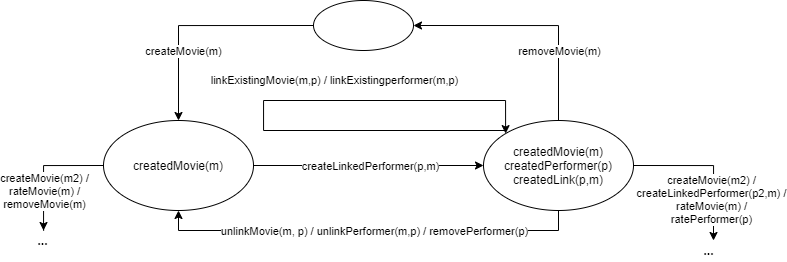
\includegraphics[width=1.0\textwidth]{img/ucts.png}
	\label{ucts}
\end{figure}

Depending on the selected coverage criterion, we receive different test objectives. How many test objectives are derived depends on the internal implementation of UCSystem and cannot be predicted for this example. Let's assume that one test objective is the test path createMovie(m) -> createLinkedPerformer(p,m) -> unlinkMovie(m). 




\subsection{An Automated Approach to System Testing based on Scenarios and Operations Contracts}


%%%%%%%%%%%%%%%%%%%%%%%%%%%%%%%%%%%%%%%%%%%%%%%%%%%%%%%%%%%%

% REFERENCES:
\newpage
\printbibliography

\end{document}

\section{Example}

In this chapter both approaches should be demonstrated within the example of a movie management software.  

\subsection{Automatic Test Generation: A Use Case Driven Approach}

In the first step the test objectives have to be derived. Therefore we define the use cases and their contracts as requirement-level logical expressions. Only the use cases that really impact the state of the transition system were specified for this example. The notation used is equal to the one proposed in the paper. 

\begin{lstlisting}
UC createMovie(m: movie)
post createdMovie(m)

UC createLinkedPerformer(p: performer, m: movie)
pre createdMovie(m)
post createdPerformer(p) and createdLink(p,m)

UC rateMovie(m: movie)
pre createdMovie(m)
post calculatedOverallRating(m)

UC ratePerformer(p: performer)
pre createdPerformer(p)
post forall(m: movie){ createdLink(p,m)@pre implies calculatedOverallRating(m) }

UC linkExistingMovie(m: movie, p: performer)
pre createdMovie(m) and createdPerformer(p)
post not createdLink(p,m)@pre implies (createdLink(p,m) and calculatedOverallRating(m))

UC linkExistingPerformer(m: movie, p: performer)
pre createdMovie(m) and createdPerformer(p)
post not createdLink(p,m)@pre implies (createdLink(p,m) and calculatedOverallRating(m))

UC unlinkMovie(m: movie, p: performer)
pre createdMovie(m) and createdPerformer(p) and createdLink(p,m)
post calculatedOverallRating(m) and not createdLink(p,m) and not exists(m2: movie){ createdLink(p,m2) }@pre implies not createdPerformer(p)

UC unlinkPerformer(m: movie, p: performer)
pre createdMovie(m) and createdPerformer(p) and createdLink(p,m)
post calculatedOverallRating(m) and not createdLink(p,m) and not exists(m2: movie){ createdLink(p,m2) }@pre implies not createdPerformer(p)

UC removeMovie(m: movie)
pre createdMovie(m)
post not createdMovie(m) and forall(p: performer){ not createdLink(p,m) } and not exist(m2: movie){ createdLink(p,m2) }@pre implies not createdPerformer(p)

UC removePerformer(p: performer)
pre createdPerformer(p)
post not createdPerformer(p) and forall(m: movie){ not createdLink(p,m) }

\end{lstlisting}

After that the UCSystem tool should build the UCTS (\autoref{ucts}) through exhaustive simulation. The pool of parameters was restricted to one movie and performer to avoid a combinatorical explosion for this example. Furthermore the predicate calculatedOverallRating is no longer considered. Note that only predicates that evaluate to true are listed in the states as in the original paper. 

\begin{figure}[h]
	\centering
	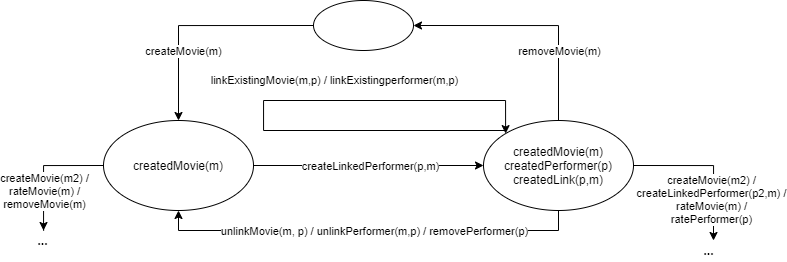
\includegraphics[width=1.0\textwidth]{img/ucts.png}
	\label{ucts}
\end{figure}

Depending on the selected coverage criterion, we receive different test objectives. How many test objectives are derived depends on the internal implementation of UCSystem and cannot be predicted for this example. Let's assume that one test objective is the test path createMovie(m) -> createLinkedPerformer(p,m) -> unlinkMovie(m). 




\subsection{An Automated Approach to System Testing based on Scenarios and Operations Contracts}


%%%%%%%%%%%%%%%%%%%%%%%%%%%%%%%%%%%%%%%%%%%%%%%%%%%%%%%%%%%%

% REFERENCES:
\newpage
\printbibliography

\end{document}
